
\documentclass[a0paper,portrait]{baposter}

\usepackage{relsize}
\usepackage{bbding}
\usepackage{pifont}

\usepackage[utf8]{inputenc} %unicode support
\usepackage[T1]{fontenc}
\usepackage{amsmath,amssymb,graphicx}
\usepackage[spanish, es-tabla]{babel}    \spanishdecimal{.}
\usepackage{float}
\usepackage{physics}
\usepackage{pifont}
				
\usepackage[dvipsnames]{xcolor}
\usepackage{setspace}
\usepackage{mwe} % new package from Martin scharrer
\usepackage{tikz,pgfplots}


\usepackage[font=tiny,labelfont=bf]{caption}
\usepackage[theorems,skins]{tcolorbox}

\usepackage{xcolor}
	\definecolor{bluemath}{rgb}{0, 1, 0}
	\definecolor{blueUNAM}{RGB}{0,60,113}
	\definecolor{orangemath}{rgb}{1, .5, .5}
	\definecolor{lblue}{RGB}{134,165,169}
	\definecolor{bluenice}{RGB}{23,176,199}
	\definecolor{gris}{RGB}{118,118,118}
	\definecolor{botwgreen1}{RGB}{83,111,80}	
	\definecolor{botwgreen2}{RGB}{146,197,130}	
	\definecolor{mxpink}{RGB}{229,0,92}	
	\definecolor{greenMathematica}{rgb}{0.560181, 0.691569, 0.194885}
%\selectcolormodel{cmyk}
	\definecolor{darkgreen}{cmyk}{0.8,0,0.8,0.45}
	\definecolor{lgreen}{cmyk}{0.8,0,0.8,0.25}

\graphicspath{{figures/}} % Directory in which figures are stoorange

\newcommand*\tick{\item[\color{mxpink}  \blacksquare ]}
\newcommand{\compresslist}{%
	\setlength{\itemsep}{0pt}%
	\setlength{\parskip}{1pt}%
	\setlength{\parsep}{0pt}%
	}

\begin{document}
\typeout{Poster rendering started}
\background{ }
\begin{poster}{
	columns = 4, 
	grid=false,
	headerborder=open, % Adds a border around the header of content boxes
	colspacing=.5em, % Column spacing
	bgColorOne=white, % Background color for the gradient on the left side of the poster
	bgColorTwo=white, % Background color for the gradient on the right side of the poster
	borderColor=white,%darkgreen, % Border color
	headerColorOne= blueUNAM, % Background color for the header in the content boxes (left side)
	headerColorTwo= bluenice, % Background color for the header in the content boxes (right side)
	headerFontColor=white,%white, % Text color for the header text in the content boxes
	%headershade= shade-tb, %plain
	boxColorOne=white, % Background color of the content boxes
	textborder=none, %rectangle, % Format of the border around content boxes, can be: none, bars, coils, triangles, rectangle, rounded, roundedsmall, roundedright or faded
	eyecatcher=true, % Set to false for ignoring the left logo in the title and move the title left
	headerheight=0.11\textheight, % Height of the header
	headershape=rectangle, % Specify the rounded corner in the content box headers, can be: rectangle, small-rounded, roundedright, roundedleft or rounded
	headerfont=\Large\textsf, % Large, bold and sans serif font in the headers of content boxes
	%textfont={\setlength{\parindent}{1.5em}}, % Uncomment for paragraph indentation
	linewidth=2pt % Width of the border lines around content boxes
}
%
%----------------------------------------------------------------------------------------
%	TITLE AND AUTHOR NAME
%----------------------------------------------------------------------------------------
%%
{\includegraphics[width=2.85cm]{../figures/image(1)}

} 
{%Titulo
	\huge{\color{blueUNAM}{ %Sans Serif
	{\noindent 
	Localización espectral de resonancias plasmónicas en nanoesferas tipo Drude de tamaño arbitrario }}}
}
{%Autores
	\normalsize%\vspace{-0.25em}\\ 
	Luna González, Dana L.$^1$, Urrutia Anguiano, Jonathan A.$^2$  y Reyes Coronado, Alejandro$^3$
	\vspace{0.1em}\\
	\footnotesize{Departamento de Física, Facultad de Ciencias, Universidad Nacional 	Autónoma de México
	\vspace{0.2em}\\
	$^1$dana.larissalg@ciencias.unam.mx,$^2$jaurrutia.95@ciencias.unam.mx, $^3$coronado@ciencias.unam.mx}
}
{\includegraphics[width=2.85cm]{../figures/image}
} %the author(s)      
%-------Resumen---------------------------
%-------abstract---------------------------
\headerbox{ \textbf{1) Resumen}}{name=abstract,column=0,row=0, span=4}{\footnotesize 
La {\color{mxpink}\textbf{nanoplasmónica}} es el estudio de la respuesta electromagnética en sistemas con respuesta metálica a la nanoescala, es decir, con dimensiones menores a 100 nm. En sistemas espacialmente confinados a esta escala, se presenta el fenómeno de {\color{mxpink}\textbf{resonancia de plasmón de superficie localizado}}, resultado del acoplamiento entre los electrones libres de un metal con el campo electromagnético incidente que ilumina al sistema. Este fenómeno se puede emplear en aplicaciones como la espectroscopía y la medicina, debido a la sintonización de dichas resonancias a una frecuencia específica según las propiedades morfológicas del sistema. En este trabajo, se estudia teórica y numéricamente la localización espectral de las resonancias plasmónicas excitadas en {\color{mxpink}\textbf{partículas esféricas}} caracterizadas por una función dieléctrica descrita por el {\color{mxpink}\textbf{modelo de Drude}} en función de su radio.
}
%-------Resumen---------------------------
%-------abstract---------------------------



%-------Introducción---------------------------
%-------intro---------------------------
\headerbox{\textbf{2) Introducción}}{name=intro,column=0,below=abstract,span=2}{\footnotesize 
La interacción de la luz con la materia es un fenómeno que tiene como consecuencia la {\color{mxpink}\textbf{absorción}} de parte de la luz incidente en la materia y el {\color{mxpink}\textbf{esparcimiento}} de luz por la materia en todas las direcciones, cuyo efecto combinado resulta en la {\color{mxpink}\textbf{extinción}} del rayo incidente \cite{Bohren}.\\

\begin{minipage}[c]{.48\linewidth}
El problema de esparcimiento de luz dada una partícula de forma, tamaño y propiedades ópticas específicas iluminada por una onda plana monocromática consiste en conocer los campos electromagnéticos en todos los puntos de la partícula y en todos los puntos del medio homogéneo en el que está embebida \cite{Bohren}. Al caso particular de esparcimiento por una partícula esférica, la solución a este problema se le conoce como {\color{mxpink}\textbf{teoría de Mie}}. Esta es una solución analítica a las ecuaciones de Maxwell que describe la excitación de la {\color{mxpink}\textbf{resonancia plasmónica de superficie}}  para partículas metálicas esféricas iluminadas por una onda electromagnética plana.\\
\end{minipage}
\begin{minipage}[c]{.5\linewidth}
	\centering
	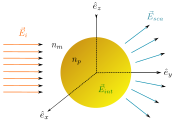
\includegraphics[width=6cm]{scattering.pdf}
	\captionof{figure}{Partícula de índice de refracción $n_p$ inmersa en un medio de índice de refracción $n_m$. La partícula es iluminada por una onda plana monocromática ($\Vec{E}_i, \Vec{H}_{i}$) que produce campos dentro ($\Vec{E}_{int}, \Vec{H}_{int}$) y fuera de la partícula ($\Vec{E}_{sca}, \Vec{H}_{sca}$).}
	\label{fig:sample_figure}
\end{minipage}	
	
Los campos EMs dentro de la partícula y los esparcidos por esta son descritos mediante coeficientes que corresponden a contribuciones multipolares de {\color{mxpink}\textbf{modos eléctricos}} y {\color{mxpink}\textbf{magnéticos}} mejor conocidos como {\color{mxpink}\textbf{coeficientes de Mie}}. En particular, los coeficientes correspondientes al campo esparcido están dados por \cite{Bohren}:
$$ {\scriptsize \tcboxmath[colback=orange!15!white ,colframe=orange,size=title]{a_n=\frac{m\psi_n(mx)\psi_n'(x)-\psi_n(x)\psi_n'(mx)}{m\psi_n(mx)\xi_n'(x)-\xi_n(x)\psi_n'(mx)}, }\hspace{0.1 cm} \tcboxmath[colback=bluenice!15!white ,colframe=blueUNAM, size=title]{b_n=\frac{\psi_n(mx)\psi_n'(x)-m\psi_n(x)\psi_n'(mx)}{\psi_n(mx)\xi_n'(x)-m\xi_n(x)\psi_n'(mx)}, }}$$ 
con $\psi_n(\rho)=\rho j_n(\rho)$ y $\xi_n(\rho)=\rho h_n^{(1)}(\rho)$ las funciones de Ricatti Bessel, $m=n_p/n_m$ y $x=2 \pi n_m/a$ el parámetro de tamaño.\\

Mediante estos, puede calcularse la {\color{mxpink}\textbf{sección transversal de extinción}} dada por \cite{Bohren}:
	$$ \tcboxmath[colback=greenMathematica!15!white ,colframe=greenMathematica,size=title]{C_{ext}=\frac{2\pi}{k^2}\sum_{n=1}^{\infty}(2n+1)\text{Re}\{a_n+b_n\}}$$
cuyo máximo corresponde a la excitación del plasmón de superficie localizado.\\

En este trabajo se propone emplear el {\color{mxpink}\textbf{método de la sección dorada}} para determinar numéricamente la posición espectral de las resonancias plasmónicas de los primeros órdenes multipolares eléctricos y magnéticos, calculando la sección transversal de extinción para cada uno de ellos, e identificando la frecuencia que maximiza estas cantidades como la resonancia plasmónica de superficie.
}
%-------Introducción---------------------------
%-------intro---------------------------



%-------CSM---------------------------
%-------csm---------------------------
\headerbox{\textbf{2) Materiales plasmónicos}}{name=mdd,column=0,below=intro,span=2}{\footnotesize 
	Cuando un material se encuentra en presencia de un campo magnético oscilante, al resolver la ecuación de movimiento que obedecen los electrones libres en el material, se obtiene la {\color{mxpink}\textbf{función dieléctrica tipo Drude}} \cite{Novotny, Ashcroft}

$$ \tcboxmath[colback=greenMathematica!15!white ,colframe=greenMathematica,size=title]{\frac{\epsilon_D(\omega)}{\epsilon_0} =1-\frac{\omega_p^2}{\omega(\omega+i\gamma)},}$$
donde $\gamma$ es la constante fenomenológica de amortiguamiento y $\omega_p$ la frecuencia de plasma.\\

 A partir de las ecuaciones de los coeficientes de Mie, se observa que, para un multipolo fijo, la contribución de los campos EMs en la sección transversal de extinción se maximiza cuando el denominador  de los coeficientes de Mie es mínimo \cite{Novotny}. Al considerar el {\color{mxpink}\textbf{límite de partícula pequeña}} ($x = k_ma \ll 1$) para esferas inmersas en vacío ($n_m = 1$),  se obtiene que los {\color{mxpink}\textbf{modos normales eléctricos}} y {\color{mxpink}\textbf{magnéticos}} cumplen las relaciones
 $$ \tcboxmath[colback=orange!15!white ,colframe=orange,size=title]{\epsilon_p(\omega_l)=-\frac{l+1}{l},}\hspace{0.5cm}\tcboxmath[colback=bluenice!15!white ,colframe=blueUNAM,size=title]{l=l-1, }$$
 respectivamente, donde se puede observar que no existe una solución para los modos normales magnéticos para ninguna $l$. Al emplear la función dieléctrica tipo Drude y considerar el límite $\gamma\rightarrow 0$, al despejar $\omega$ se obtiene la  expresión para la frecuencia de resonancia del modo normal eléctrico del multipolo $l$ dada por
$$ \tcboxmath[colback=orange!15!white ,colframe=orange,size=title]{\frac{\omega_l}{\omega_p}=\sqrt{\frac{l}{2l+1}}.}$$
}
%-------CSM---------------------------
%-------csm---------------------------

%-------modo plasmónico guiado---------------------------
%-------nmodo---------------------------
%-------modo plasmónico guiado---------------------------
%-------nmodo---------------------------

%-------modo plasmónico guiado---------------------------
%-------nmodo---------------------------
\headerbox{\textbf{4) Resultados}}{name=nmodo,span=2,column=2,below=abstract}{\footnotesize
	Las resonancias de los materiales plasmónicos dependen del
	parámetro adimensional $\tilde{a}=\omega_p a/c$, que compara la frecuencia de excitación $\omega$ con el
	tiempo de acoplamiento $ac^{-1}$ entre la interacción EM de la esfera y la densidad de carga
	inducida que corresponde al plasmón de superficie \cite{Aizpurua}. Por ello, se reescribieron los coeficientes de Mie, en términos de esta interacción, considerando las siguientes definiciones
	$$n_p=\sqrt{1-\frac{1}{\tilde{\omega}(\tilde{\omega}+i\tilde{\gamma})}},\hspace{1cm}x=\tilde{\omega}\tilde{a}n_m.$$	
	
	En las siguientes figuras se muestran las contribuciones individuales de las secciones transversales de extinción de los multipolos $l = 1, 2, 3, 4$, $5$ eléctricos y magnéticos, en términos del parámetro $\tilde{\omega}$ y  $\tilde{\gamma}$, donde se consideró $\tilde{a}=5,n_m=1,
\tilde{\gamma} =\gamma/\omega_p\approx 10^{-2}$.\\

Además, se muestran las frecuencias de resonancia $\omega_l$ normalizadas respecto a la frecuencia de plasma $\omega_p$, como función del parámetro adimensional $\omega_p a/c$ para los multipolos $l = 1, 2, 3, 4$ y $5$.\\

\begin{tikzpicture}
	\node at (-2.5,5) {\footnotesize \textbf{Eléctricos}};
	\node at (3,5) {\footnotesize \textbf{Magnéticos}};
\node[inner sep=0pt] (graf) at (0,1){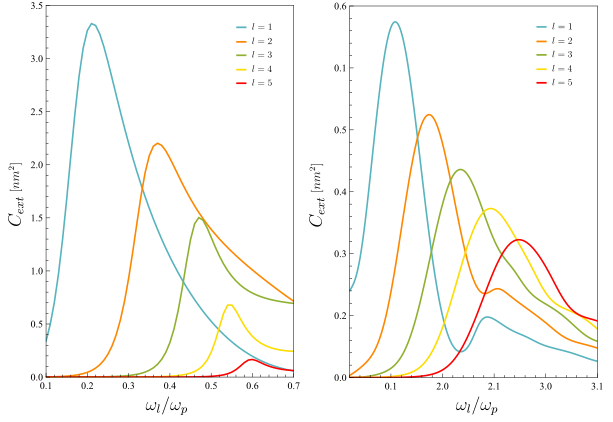
\includegraphics[scale=.5]{SeccTrans2.pdf}};
\node[inner sep=0pt] (graf) at (0,-4.5){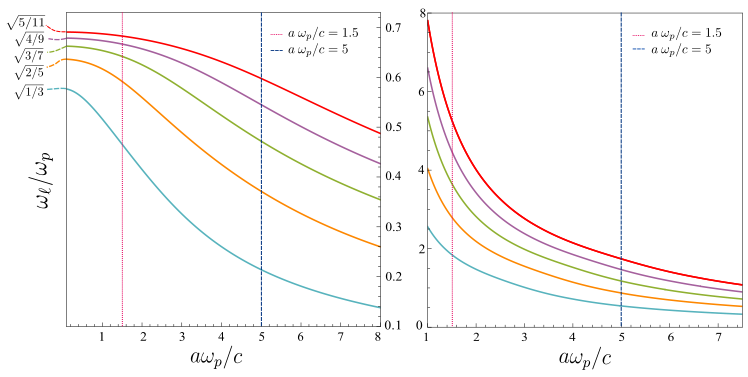
\includegraphics[scale=.57]{Resonances.pdf}};
\end{tikzpicture}


}

\headerbox{\textbf{5) Conclusiones}}{name=conclusiones,column=2,below=nmodo,span=2}{
	\footnotesize
	\begin{itemize}
		\tick La banda de frecuencias en la que las frecuencias de resonancia de los modos eléctricos se espera que se encuentren es $[\omega_{p}/\sqrt{3},\omega_{p}/\sqrt{2}]$, cuyos límites corresponden al modo plasmónico dipolar eléctrico y a la resonancia plasmónica de superficie de una esfera de radio infinito, es decir, a un plano infinito.
		\tick Conforme el límite de partícula pequeña deja de ser válido se presenta un corrimiento al rojo de las resonancias plasmónicas de superficie localizadas de los modos eléctricos y magnéticos para partículas esféricas.
		\tick No es posible calcular una aproximación de las frecuencias de resonancia de los modos normales magnéticos en el límite de partícula pequeña.
	\end{itemize}
}
%-------modo plasmónico guiado---------------------------
%-------nmodo---------------------------





\headerbox{\textbf{6) Referencias}}{name=references,column=2,span=2,below=conclusiones}{
\renewcommand{\section}[2]{\vskip 0.05em} % Get rid of the default "References" section title
\begin{thebibliography}{99} \scriptsize \compresslist
\bibitem{Bohren} C.F. Bohren y D.R. Huffman , \textit{Absorption and scattering of light by small particles} (John Wiley \& Sons, 1980). 
\bibitem{Novotny} L. Novotny, \textit{Principles of Nano-Optics} (Cambridge University Press, New York, 2006). 
\bibitem{Ashcroft} N.W. Ashcroft y N.D. Mermin, \textit{Solid State Physics}, \textit{Principles of Nano-Optics} (Saunders College, 1976). 
\bibitem{Aizpurua} J. Aizpurua, \textit{Coupling of electrons and electromagnetic surface modes in scanning transmission electron microscopy} (Tesis doctoral, Universidad de País Vasco, País Vasco, España,
1998). 
\end{thebibliography}\footnotesize
}

\headerbox{{\scriptsize Agradecimientos al proyecto PAPIIT-UNAM IN107122 y a la Facultad de Ciencias de la UNAM}}{name=thaks,column=2,span=2,below=references}{ \hfill}

\end{poster}

\end{document}
